\documentclass[12pt]{article}
% Эта строка — комментарий, она не будет показана в выходном файле
\usepackage{ucs}
\usepackage[warn]{mathtext} 
\usepackage[utf8x]{inputenc} % Включаем поддержку UTF8
\usepackage[russian]{babel}  % Включаем пакет для поддержки русского языка
\usepackage{amsmath}
\usepackage{mathtools}
\usepackage{amssymb}
% \usepackage[dvips]{graphicx}
% \graphicspath{{noiseimages/}}
\usepackage[pdftex]{graphicx}

\hoffset=0mm
\voffset=0mm
\textwidth=180mm        % ширина текста
\oddsidemargin=-6.5mm   % левое поле 25.4 - 5.4 = 20 мм
\textheight=240mm       % высота текста 297 (A4) - 40
\topmargin=-15.4mm      % верхнее поле (10мм)
\headheight=5mm      % место для колонтитула
\headsep=5mm          % отступ после колонтитула
\footskip=8mm         % отступ до нижнего колонтитула


\begin{document}
	\author {Жарков Андрей 496}
	\title {Лабораторная работа 1.4 \\ Исследование вынужденной прецессии
		гироскопа}
	\maketitle{}
	
	\indent
	\textbf{Цель работы:} исследовать вынужденную прецессию уравновешенного симметричного гироскопа; установить зависимость угловой скорости вынужденной прецессии от величины момента сил, действующих на ось гироскопа; по угловой скорости прецессии определить
	угловую скорость вращения ротора гироскопа
	\\\newline
	\indent
	\textbf{В работе используются:} гироскоп в кардановом подвесе, секундо-
	мер, набор грузов, отдельный ротор гироскопа, цилиндр известной
	массы, крутильный маятник, штангенциркуль, линейка.
	\\\newline
	
	\textbf{Определение.} Гироскопом называют быстро вращающееся твёрдое тело, ось вращения которого способна изменять своё положение в пространстве. Простейшим повседневным примером гироскопа является детский волчок.
	В данной работе рассматривается широко применяемый в технике роторный гироскоп. Характерным свойством таких устройств является
	стабильность оси вращения, которая обеспечивается законом сохранения вращательного момента (момента импульса).
	
	Произвольное вращение твёрдого тела с одной неподвижной точкой
	описывается уравнением моментов: 
	\begin{equation}
	\frac{d\vec{L}}{dt} = \vec{M}
	\end{equation}
	
	Мы будем рассматривать один из простейших случаев — движение
	симметричного волчка, закреплённого в центре масс (такой гироскоп
	называют уравновешенным), быстро вращающегося вокруг своей оси
	симметрии.
	
	Любое движение твёрдого тела, имеющего одну неподвижную точку,
	можно рассматривать как вращение вокруг мгновенной оси, проходящей через эту точку. С течением времени мгновенная ось может перемещаться как в теле, так и в пространстве.
	
	Для описания вращения вводится вектор угловой скорости $\vec{\omega}$. Его модуль задаёт темп изменения угла поворота, а направление — мгновенную ось вращения согласно правилу правого винта.
	
	Движение осесимметричного тела удобно разбить на две составляющие — выделить из вектора полной угловой скорости $\vec{\omega}$  угловую скорость вращения оси симметрии $\vec{\Omega}$, которую обычно называют угловой	скоростью прецессии, и $\vec{\omega_0}$ — угловую скорость «собственного» вращения:
	\begin{equation}
	\vec{\omega} = \vec{\omega_0} + \vec{\Omega}
	\end{equation}
	
	Вектор $\Omega$ в рассматриваемом нами случае (осесимметричный волчок) может быть разложен ещё на две составляющие: вдоль оси симметрии и перпендикулярно ей $\vec{\Omega} = \vec{\Omega}_{||}+\vec{\Omega}_{\perp}$	Тогда момент импульса ротора гироскопа также представится в виде суммы своих составляющих: продольной и поперечной
	\begin{equation}
	\vec{L} = \vec{L}_{||} + \vec{L}_{\perp} = \vec{I}_{||} \left( \vec{\omega}_0 + \vec{\Omega}_{||} \right) + I_{\perp} \vec{\Omega}_{\perp}
	\end{equation}
	
	Откуда при быстром вращении $\vec{L} = I_{||} \vec{\omega}_0$
	Если же приложить к исходно уравновешенному гироскопу внешнюю силу с ненулевым моментом $\vec{M}$
	
	Уравнение вращательного движения (1) легко решается в «гироскопическом» приближении, т. е. в предположении, что весь момент
	импульса $\vec{L}$ ротора гироскопа направлен вдоль его оси симметрии. При
	этом $\vec{L}$ будет вращаться вместе с осью гироскопа $\vec{s}$ с некоторой
	угловой скоростью $\vec{\Omega}$, которая должна быть много меньше скорости собственного вращения.
	
	Для нахождения уравнения движения оси гироскопа воспользуемся следующей аналогией: если некоторый радиус-вектор $\vec{r}$ вращается с
	угловой скоростью $\vec{\Omega}$, то линейная скорость движения его конца равна $$\vec{v} = \frac{d\vec{r}}{dt} = \vec{\Omega} \times \vec{r}$$
	Следовательно, движение оси определяется аналогичным соотношением: уравнение вращения вектора $\vec{s}$ есть
	\begin{equation}
	\frac{d\vec{s}}{dt} = \vec{\Omega} \times \vec{s}
	\end{equation}
	Тогда с учётом базового уравнения моментов (1) и приближения
	получим основное уравнение вынужденной регулярной прецессии гироскопа:
	\begin{equation}
	\vec{\Omega} \times \vec{L} = \vec{M}
	\end{equation}
	Отсюда выражаем угловую скорость прецессии:
	\begin{equation}
	\Omega = \frac{M}{Lsin\angle(\vec{L}\vec{\Omega})} = \frac{mgrcos\alpha}{I_0 \omega_0 sin(\pi/2 - \alpha)} = \frac{mgr}{I_0 \omega_0}
	\end{equation}
	\begin{center} 
		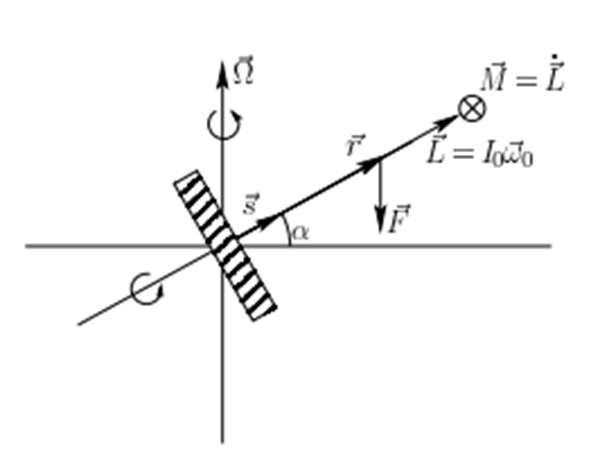
\includegraphics[width=3in]{4_1.png} \\ Рис. 1: прецессия под действием груза $\vec{F} = m\vec{g}$
	\end{center}
	Вектор $\vec{\Omega}$ направлен вертикально, т. е. гироскоп под действием веса грузика придёт во вращение вокруг вертикальной оси, а скорость этого
	вращения не зависит от угла наклона оси гироскопа к горизонтали.
	По времени оборота гироскопа в процессе регулярной прецессии можно
	определить угловую скорость вращения ротора.
	
	\textbf{Экспериментальная установка.} Для закрепления гироскопа в его
	центре масс (уравновешенный гироскоп) в данной работе используется
	карданов подвес, показанный на рис. 3. Наружное кольцо подвеса А может свободно поворачиваться вокруг вертикальной оси аа. Внутреннее кольцо Б связано с кольцом А горизонтальной осью бб. В кольце Б укреплен гироскоп, ось вращения которого вв перпендикулярна к оси бб. Центр масс гироскопа находится на пересечении всех трех осей и при любом повороте колец сохраняет свое положение в пространстве.
	\begin{center} 
		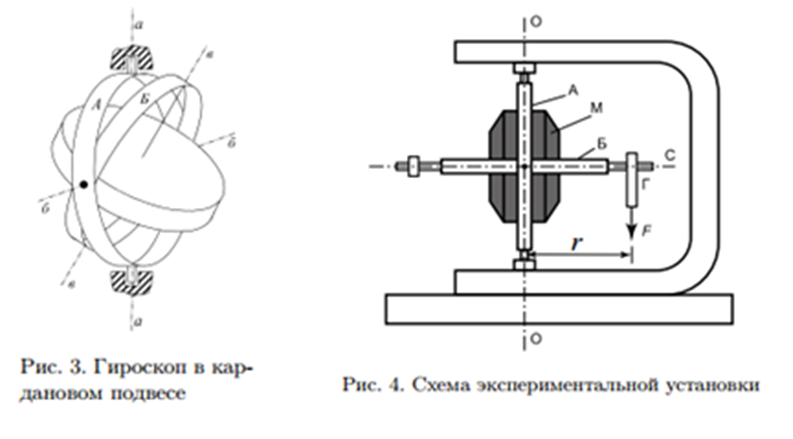
\includegraphics[width=5in]{4_2.png}
	\end{center}
	Экспериментальная установка для исследования прецессии уравновешенного гироскопа показана на рис. 4. Ротором гироскопа является
	ротор высокооборотного электромотора М, питающегося током частотой 400 Гц. Кожух мотора (статор, имеющий обмотки, питаемые током
	частотой 400 Гц) скреплен с кольцом Б. Мотор с
	кольцом Б может вращаться в кольце А вокруг
	горизонтальной оси бб, которое может вращаться вокруг вертикальной оси аа. Ротор электромотора представляет массивный стальной цилиндр с прожилками меди, образующими «беличье колесо». Обозначенный на рис. 4 буквой С рычаг направлен по оси симметрии ротора. На рычаг подвешивают грузы Г. Подвешивая различные грузы, можно изменять силу 𝐹, момент которой определяется расстоянием 𝑟 от точки подвеса до горизонтальной оси кольца А (до центра
	масс гироскопа), указанным на самой установке.
	\\ \\
	\textbf{\large Выполнение работы}
	\\ \\
	Для начала вычислим момент инерции гироскопа относительно оси вращения: $$I_0 = I_ц \frac{T_0^2}{T_ц^2},$$ где $I_ц = \frac{m_ц d^2}{8}$, $T_0$ - период крутильных колебаний гироскопа, $T_ц$ - период крутильных колебаний цилиндра.
	$m_ц$ = 1617,7 г,
	$d$ = 7,8 см,
	$T_0$ = $\frac{90.2 \pm 0.3 c}{15} = 6.01 \pm 0.02 c$,
	$T_ц$ = $\frac{72.0 \pm 0.3 c}{15} = 4.80 \pm 0.02 c$
	Откуда $I_0 = (7.84 \pm 0.13)*10^{-4}$ $кг*м^2$
	
	По реакции гироскопа на приложенную к рычагу силу $\vec{F}$ легко определить как вращается гироскоп (см. рис)
	\begin{center} 
		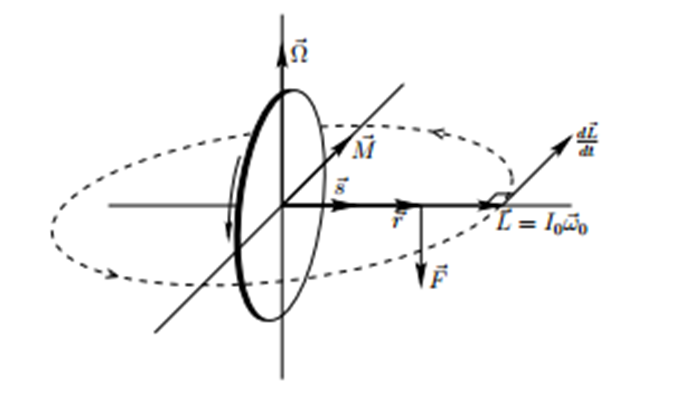
\includegraphics[width=3in]{4_5.png}
	\end{center}
	Далее представлены результаты измерений различных величин при подвешивании на рычаг грузов различной массы
	\begin{center} 
		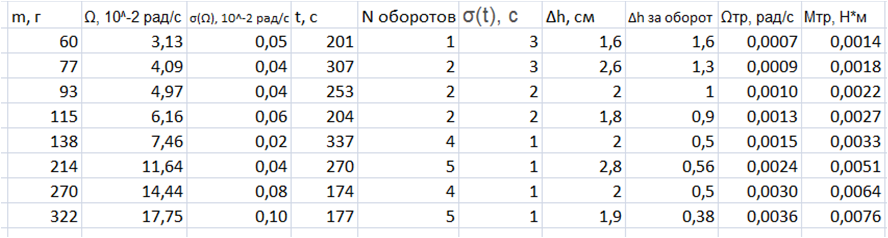
\includegraphics[width=4in]{4_3.png}
	\end{center}
	Построим график зависимости угловой скорости $\Omega$ от массы $m$ груза
	\begin{center} 
		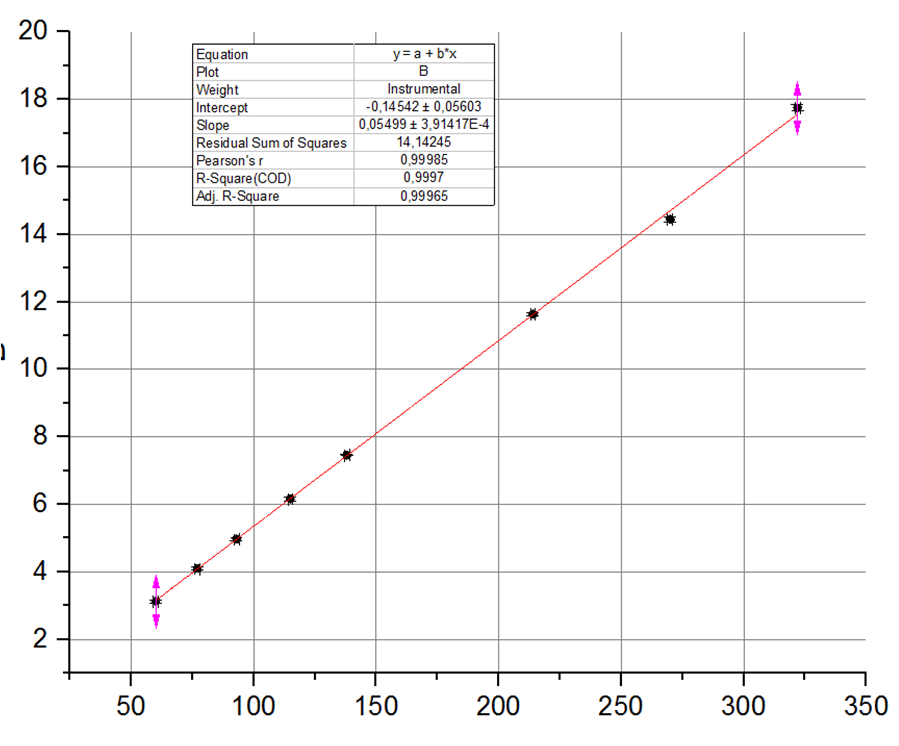
\includegraphics[width=5in]{4_4.png}
	\end{center}
	Как видим, график линейный с хорошей точностью: $\Omega = km$, где $k = (5.49 \pm 0.04) * 10^{-1}$ $\frac{рад}{с*кг}$
	С другой стороны, по формуле (6) $k = \frac{gr}{I_0 \omega_0}$ \\
	Откуда $\omega_0 = \frac{gr}{I_0 k} = (274 \pm 3)*10 \frac{рад}{c} $ \\
	Что в пределах погрешности равняется $\omega = 2\pi\nu = 2760 \frac{рад}{c}$
	($\nu = 439 Гц$) \\
	Мы убедились, что в данной работе приближение $\vec{L} = I_{||}\vec{\omega_0}$ допустимо.
	
	
\end{document}